\title{Лекция 15\\Структуризация баз знаний на основе иерархии онтологий}
\author[]{Шункевич Д.В.}
\institute[]{Белорусский государственный университет информатики и радиоэлектроники}

\begin{frame}
	\titlepage
\end{frame}

\begin{frame}{\\Содержание лекции}
	\topline
	\justifying
	Понятие раздела базы знаний. Типология разделов, иерархия разделов. Атомарные и неатомарные разделы, декомпозиция разделов, дочерний раздел. Предметные области и онтологии верхнего уровня, их взаимосвязь.
\end{frame}

\begin{frame}{\\Структуризация базы знаний}
	\topline
	\justifying
	\begin{SCn}
		\textbf{Аспекты структуризации базы знаний}
		\begin{textitemize}
			\item  иерархия предметных областей и онтологий
			\item дидактическая (логическая) структуризация
			\item структуризация с точки зрения процесса разработки
		\end{textitemize}
	\scnheader{дидактическая структуризация}
	\scnidtf{структуризация с точки зрения восприятия конечным пользователем}
	\scntext{примечание}{Дидактическая структуризация не должна искажать знания.}
	\end{SCn}
\end{frame}

\begin{frame}{\\Понятие раздела базы знаний}
	\topline
	\justifying
	База знаний каждой ostis-системы декомпозируется на разделы.\\
	Понятие раздела представляет собой знак	множества всевозможных разделов, входящих в	состав различных баз знаний. \\ \vspace{10mm}
	Каждый раздел является условно \textit{дидактически} выделяемым	фрагментом базы знаний, обладающим \textit{логической	целостностью и завершенностью.}\\
	Вся база знаний	конкретной ostis-системы также может	рассматриваться как один неатомарный раздел.
\end{frame}

\iffalse
\begin{frame}{\\Отношение, заданные на понятии раздела}
	\topline
	\justifying
	\begin{SCn}
		\scnheader{отношения на множестве разделов}
		\scnhaselement{декомпозиция раздела*}
			\begin{scnindent}
				\scnidtf{квазибинарное ориентированное отношение между разделом и множеством его подразделов}
				\scnidtf{отношение, задающее дидактическую структуру раздела}
				\scntext{примечание}{В отличие от отношения базовая декомпозиция*, которое	связывает некоторую \textbf{сущность} с другими \textbf{сущностями}, являющимися её частями, отношение декомпозиция раздела* связывает \textbf{раздел} с его \textbf{подразделами}, т.е. сужается область определения отношения базовая декомпозиция*}
			\end{scnindent}
		\scnhaselement{базовый порядок разделов*}
			\begin{scnindent}
				\scnidtf{бинарное отношение между разделами, определяющее порядок их следования в рамках декомпозиции	раздела}
			\end{scnindent}
		
	\end{SCn}
\end{frame}
\fi

\begin{frame}{\\Типология разделов базы знаний}
	\topline
	\justifying
	\begin{SCn}
		\scnheader{раздел}
		\scnidtf{раздел базы знаний}
		\begin{scnrelfromset}{разбиение}
			\scnitem{неатомарный раздел}
			\scnitem{атомарный раздел}
		\end{scnrelfromset}
		\scnsuperset{раздел-обоснование}
		\scnsuperset{раздел-описание принципов}
		\scnsuperset{раздел-документация}
		\scnsuperset{раздел-описание предметной области}
		\scnsuperset{раздел-описание семантической окрестности}
	\end{SCn}
\end{frame}

\begin{frame}{\\}
	\topline
	\justifying
	\begin{SCn}
		\scnheader{раздел-обоснование}
		\scnidtf{формальный текст, обосновывающий разработку чего-либо, то есть постановку проблемы, указание недостатков существующих решений, достоинства предлагаемых решений и т.д.}
		
		\scnheader{раздел-описание принципов}
		\scnidtf{описание основополагающих принципов устройства	либо функционирования технологии, подсистемы и т.д}
		
		\scnheader{раздел-документация}
		\scnidtf{описание назначения системы или подсистемы, принципов работы с той или иной системой или подсистемой, ее структуры и состава}
	\end{SCn}
\end{frame}

\begin{frame}{\\}
	\topline
	\justifying
	\begin{SCn}

		\scnheader{раздел-описание предметной области}
		\scnidtf{раздел, содержащий знак самой этой ПрО, знаки всех ее элементов, а также всю спецификацию этой ПрО, включая	все ее онтологии}
		
		\scnheader{раздел-описание семантической окрестности}
		\scnidtf{раздел, содержащий знак структуры, которая	является семантической окрестностью некоторого sc-элемента, знаки всех ее элементов, а так же	спецификацию этой структуры}
	\end{SCn}
\end{frame}


\begin{frame}{Понятия атомарного и неатомарного\\ разделов}
	\topline
	\justifying
	
Под неатомарным разделом понимается знак множества всевозможных неатомарных разделов, входящих в состав различных документаций, т. е. разделов, которые декомпозируются на более частные разделы. Вся база знаний конкретной ostis-системы также может рассматриваться как один неатомарный раздел.
\bigskip
Соответственно, под атомарным разделом понимается знак множества всевозможных атомарных разделов, входящих в состав различных документации, т. е. разделов, не декомпозируемых на более частные разделы. Любое понятие, входящее в состав атомарного раздела и не являющееся ключевым в рамках этого раздела, должно стать ключевым в рамках какого-либо другого атомарного раздела рассматриваемой базы знаний. \\
\end{frame}

\begin{frame}{\\Иерархия разделов}

	\topline
	\justifying
	\begin{SCn}
		\scnheader{раздел базы знаний}
		\scntext{примечание}{Иерархия разделов базы знаний задается отношениями \textit{частная предметная область*}, \textit{частная предметная область и онтология*}, \textit{дочерний раздел*}}
		
		\scnheader{Раздел. ПрО знаний и баз знаний}
		\scnrelfrom{дочерний раздел}{Раздел. ПрО множеств}
	\end{SCn}
\end{frame}

\begin{frame}{\\Фрагмент базы знаний}
	\topline
	\justifying
	\begin{SCn}
		 \scnheader{выделенный фрагмент базы знаний}
			 \begin{scnrelfromset}{разбиение}
			 	\scnitem{семейство разделов базы знаний}
			 	\scnitem{раздел базы знаний}
			 	\scnitem{сегмент базы знаний}
			 	\scnitem{фрагмент базы знаний}
			 \end{scnrelfromset}	
	 	 \scnheader{раздел базы знаний}
		 	 \begin{scnrelfromset}{разбиение}
		 	 	\scnitem{атомарный раздел базы знаний}
		 	 	\scnitem{неатомарный раздел базы знаний}
		 	 		\begin{scnindent}
		 	 			\scnidtf{раздел, который делится на сегменты}
		 	 		\end{scnindent}
		 	 \end{scnrelfromset}
	\end{SCn}
\end{frame}

\begin{frame}{\\Раздел, сегмент, фрагмент базы знаний}
	\topline
	\justifying
	\begin{SCn}
		\scnheader{раздел базы знаний}
		\scnsuperset{предметная область и онтология}
		\scnsuperset{фрагмент предметной области}
		\scnsuperset{частная онтология}
		\scnsuperset{интегрированная онтология}
		\scnsuperset{предметная область}
		
		\scnheader{сегмент базы знаний}
		\scnidtf{часть неатомарного раздела базы знаний}
		\scntext{примечание}{Сегменты базы знаний не могут иметь иерархической структуры, т.е. не могут состоять из сегментов более низкого уровня.}
		
		\scnheader{фрагмент базы знаний}
		\scnidtf{часть раздела базы знаний}
	\end{SCn}
\end{frame}

\begin{frame}{\\}
	\topline
	\justifying

	\vspace{3em}
	\begin{SCn}
		\begin{figure}[H]
			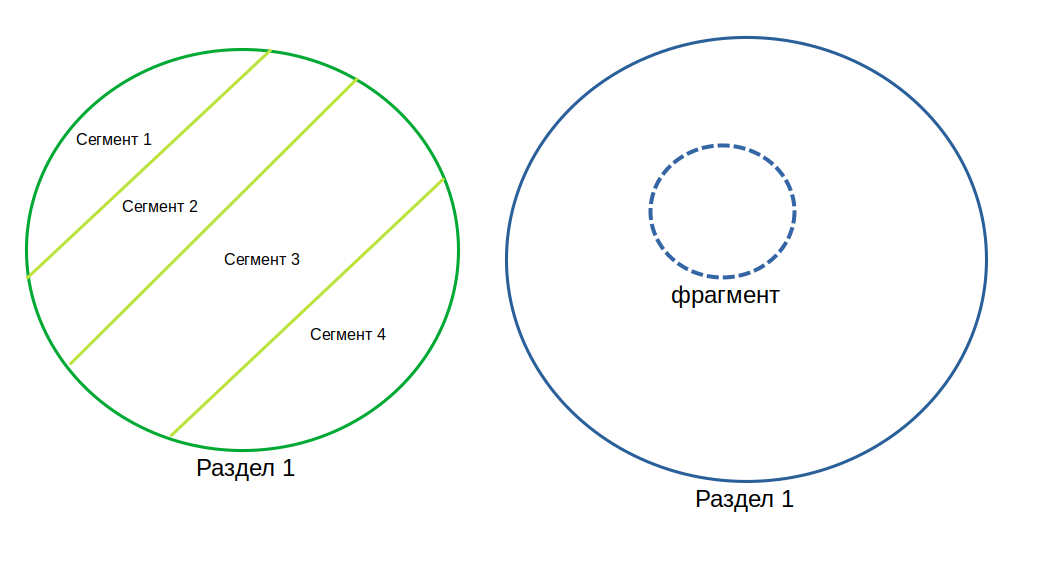
\includegraphics[scale=0.2]{./figures/sd_structuring/segment.png}
		\end{figure}
	\vspace{-1em}
	\begin{columns}[T,onlytextwidth]
		\begin{column}{0.4\textwidth}

				\scnheader{Раздел 1}
				\begin{scnreltoset}{покрытие}
					\scnitem{Сегмент 1}
					\scnitem{Сегмент 2}
					\scnitem{Сегмент 3}
					\scnitem{Сегмент 4}
				\end{scnreltoset}

		\end{column}
		\begin{column}{0.4\textwidth}
			\scnheader{Раздел 1}
			\scnsuperset{фрагмент}
		\end{column}
	\end{columns}
	\end{SCn}
\end{frame}


\begin{frame}{\\Выделенный фрагмент базы знаний}
	\topline
	\justifying
	\begin{SCn}
		\scnheader{выделенный фрагмент базы знаний}
		\begin{scnrelfromset}{разбиение}
			\scnitem{именованный фрагмент базы знаний}
				\begin{scnindent}
					\scnsuperset{раздел базы знаний}
					\scnsuperset{сегмент базы знаний}
				\end{scnindent}
			\scnitem{неименованный фрагмент базы знаний}
		\end{scnrelfromset}
	\scnheader{семейство разделов базы знаний}
	\scnidtf{множество разделов базы знаний}
	
	\scnheader{неатомарный раздел базы знаний}
	\scnidtf{раздел, не являющийся множеством сегментов базы знаний}
	\end{SCn}
\end{frame}

\begin{frame}{\\Пример}
	\topline
	\justifying
	\begin{SCn}
		\scnheader{многоугольники}
		\scniselement{семейство разделов}
		\begin{scneqtoset}
			\scnitem{Треугольники\\
			\begin{scnindent}
				\scniselement{неатомарный раздел базы знаний}
				\begin{scnreltoset}{контакенация сегментов}
					\scnitem{Классификация треугольников}
					\scnitem{Отношения на треугольниках}
					\scnitem{Свойства треугольников}
				\end{scnreltoset}
			\end{scnindent}}
			\scnitem{Четырехугольники\\
			\begin{scnindent}
				\scniselement{атомарный раздел}
			\end{scnindent}}
			\scnitem{Правильные многоугольники\\
				\begin{scnindent}
					\scniselement{атомарный раздел}
				\end{scnindent}}
		\end{scneqtoset}
	\end{SCn}
\end{frame}

\begin{frame}{Отношения на множестве выделяемых фрагментов}
	\topline
	\justifying
	\begin{SCn}
		\scnheader{отношения на множестве выделяемых фрагментов}
		\scnhaselement{конкатенация сегментов*}
		\scnhaselement{дочерний фрагмент базы знаний*}
			\begin{scnindent}
				\scnsuperset{дочерний фрагмент раздела базы знаний*}
				\scnsuperset{дочерний раздел базы знаний*}
				\begin{scnindent}
					\scntext{примечание}{\textit{дочерний раздел базы знаний*} не одно и то же, что \textit{включение*} или \textit{частная предметная область*}}
				\end{scnindent}
			\end{scnindent}
	\end{SCn}
\end{frame}

\begin{frame}{\\}
	\topline
	\justifying
	\begin{SCn}
		\scnheader{отношения на множестве выделяемых фрагментов}
		\scnhaselement{аннотация*}
		\scnhaselement{предисловие*}
		\scnhaselement{введение*}
		\scnhaselement{заключение*}
		\scnhaselement{выводы*}
		\scnhaselement{эпиграф*}
		
		\scnheader{отношения дидактического характера}
		\scnhaselement{пояснение*}
		\scnhaselement{примечание*}
		\scnhaselement{сходства*}
		\scnhaselement{сравнение*}
		\scnhaselement{отличие*}
		\scnhaselement{следует отличать*}
	\end{SCn}
\end{frame}

\begin{frame}{\\}
	\topline
	\justifying
	\begin{SCn}
		\scnheader{отношения дидактического характера}
		\scntext{пояснение}{Такие отношения являются избыточными, т.е. реальной необходимости в них нет, но с использование данных отношений позволяет представить знания более понятным способом для пользователя.}
	\end{SCn}
\end{frame}


\begin{frame}{\\Предметные области верхнего уровня}
	\topline
	\justifying
	
	В предметных областях верхнего уровня классами объектов исследования являются наиболее общие (широкие) классы сущностей (категории). \\
	Например:
	\begin{textitemize}
		\item класс всевозможных параметров
		\item класс всевозможных структур
		\item класс всевозможных связей
		\item класс всевозможных множеств
		\item класс знаний всевозможного вида
	\end{textitemize}

	Каждой предметной области можно поставить в соответствие онтологии разного вида, которые уточняют смысл понятий (описывают их).
\end{frame}

\begin{frame}{\\Онтологии верхнего уровня}
	\topline
	\justifying
	 Онтология, поставленная в соответствие предметной области верхнего уровня, называется онтологией верхнего уровня. В онтологии верхнего уровня представлена систематизация знаний о реальном мире безотносительно к какой-либо конкретной предметной области. \\\vspace{3mm}
	 Основной функцией, которая возлагалась на онтологии верхнего уровня, является поддержка семантической совместимости онтологий предметных областей и прикладных онтологий. Поддержка предполагает создание общей точки для формулирования определений. Термины предметно-ориентированных онтологий подчинены терминам онтологии более высокого уровня. \\
\end{frame}